\documentclass[12pt, titlepage]{article}

\usepackage{booktabs}
\usepackage{tabularx}
\usepackage{hyperref}
\hypersetup{
    colorlinks,
    citecolor=black,
    filecolor=black,
    linkcolor=red,
    urlcolor=blue
}
\usepackage[round]{natbib}
\usepackage{geometry}

\usepackage{adjustbox}
\usepackage[dvipsnames]{xcolor}
\usepackage{float}
\usepackage{changepage}
\usepackage{pdflscape}

%% Comments

\usepackage{color}

\newif\ifcomments\commentstrue %displays comments
%\newif\ifcomments\commentsfalse %so that comments do not display

\ifcomments
\newcommand{\authornote}[3]{\textcolor{#1}{[#3 ---#2]}}
\newcommand{\todo}[1]{\textcolor{red}{[TODO: #1]}}
\else
\newcommand{\authornote}[3]{}
\newcommand{\todo}[1]{}
\fi

\newcommand{\wss}[1]{\authornote{blue}{SS}{#1}} 
\newcommand{\plt}[1]{\authornote{magenta}{TPLT}{#1}} %For explanation of the template
\newcommand{\an}[1]{\authornote{cyan}{Author}{#1}}

%% Common Parts

\newcommand{\progname}{Software Engineering} % PUT YOUR PROGRAM NAME HERE
\newcommand{\authname}{Team \#13, ARC
    \\ Avanish, Ahluwalia
    \\ Russell, Davidson
    \\ Rafey, Malik
    \\ Abdul, Zulfiqar} % AUTHOR NAMES                  

\usepackage{hyperref}
    \hypersetup{colorlinks=true, linkcolor=blue, citecolor=blue, filecolor=blue,
                urlcolor=blue, unicode=false}
    \urlstyle{same}
                                


\begin{document}

\title{Verification and Validation Report: \progname}
\author{\authname}
\date{March 10, 2025}

\maketitle

\pagenumbering{roman}

\section{Revision History}

\begin{tabularx}{\textwidth}{p{3cm}p{2cm}X}
  \toprule {\bf Date} & {\bf Version} & {\bf Notes} \\
  \midrule
  Date 1              & 1.0           & Notes       \\
  Date 2              & 1.1           & Notes       \\
  \bottomrule
\end{tabularx}

~\newpage

\section{Symbols, Abbreviations and Acronyms}

\renewcommand{\arraystretch}{1.2}
\begin{tabular}{l l}
  \toprule
  \textbf{symbol} & \textbf{description} \\
  \midrule
  T               & Test                 \\
  \bottomrule
\end{tabular}\\

\newpage

\tableofcontents

\listoftables %if appropriate

\listoffigures %if appropriate

\newpage

\pagenumbering{arabic}

This document ...

\section{Functional Requirements Evaluation}

\subsection{Profile Testing}
The following section presents the results of the profile testing


\begin{table}[H]
  \caption{\bf Functional Requirements Evaluation Results for Profile Testing}
  \resizebox{6in}{!}{\begin{tabular}{|l|p{0.15\linewidth}|p{0.3\linewidth}|p{0.3\linewidth}|p{0.3\linewidth}|p{0.1\linewidth}|}
      \hline
      \multicolumn{1}{|l|}{\bfseries Id} & \multicolumn{1}{|l|}{\bfseries Type} & \multicolumn{1}{l|}{\bfseries Inputs}                                      & \multicolumn{1}{l|}{\bfseries Expected Result}                              & \multicolumn{1}{l|}{\bfseries Actual Result} & \multicolumn{1}{l|}{\bfseries Result} \\
      \hline
      Test-PS1                           & Manual                            & User enters valid credentials.                                          &  The user successfully logs in and
is redirected to their profile page. & Same as expected                             & \textcolor{Green}{Pass}               \\
      \hline
      Test-PS2                           & Manual                            & User inputs new password and confirms. & System updates the password
and provides a confirmation message.                        & Same as expected                             & \textcolor{Green}{Pass}               \\
      \hline
    Test-PS3                           & Automated                            & None & Profile information (username,
password, status) is displayed correctly.                        & Same as expected                             & \textcolor{Green}{Pass}               \\
      \hline
    Test-PS4                           & Manual                            & User navigates to help page. & A help page with FAQs and ad-
ditional help information is displayed.                        & Same as expected                             & \textcolor{Green}{Pass}               \\
      \hline
    \end{tabular}}
\label{table:GR7}
\end{table}

\subsection{Touring}
The following section presents the results of the general users experience of using a tour.


\begin{table}[H]
  \caption{\bf Functional Requirements Evaluation Results for Touring}
  \resizebox{6in}{!}{\begin{tabular}{|l|p{0.15\linewidth}|p{0.3\linewidth}|p{0.3\linewidth}|p{0.3\linewidth}|p{0.1\linewidth}|}
      \hline
      \multicolumn{1}{|l|}{\bfseries Id} & \multicolumn{1}{|l|}{\bfseries Type} & \multicolumn{1}{l|}{\bfseries Inputs}                                      & \multicolumn{1}{l|}{\bfseries Expected Result}                              & \multicolumn{1}{l|}{\bfseries Actual Result} & \multicolumn{1}{l|}{\bfseries Result} \\
      \hline
      Test-TR1                           & Manual                            & General user attempts to navigate to the touring screen.                                          &  The touring screen is reachable. & Same as expected                             & \textcolor{Green}{Pass}               \\
      \hline
      Test-TR2                           & Manual                            & Organization user attempts to navigate to touring screen. & The touring screen is hidden from user.                        & Same as expected                             & \textcolor{Green}{Pass}               \\
      \hline
    Test-TR3                           & Manual                            & General user finds a tour and attempts to preview it & User can see the information described in TR-FR3.                        & Same as expected                             & \textcolor{Green}{Pass}               \\
      \hline
    Test-TR4                           & Manual                            & General user navigates to the tour list interface, and searches for a tour
belonging to an organization. & The tour has been found.                      & Same as expected                             & \textcolor{Green}{Pass}               \\
      \hline
    Test-TR5                           & Manual                            & General user goes close to a tour area in the real-world & A push notification appears on the user’s phone indicating
that a tour is nearby and prompts them to preview it.                      & Same as expected                             & \textcolor{Green}{Pass}               \\
        \hline
      Test-TR6                           & Manual                            & General user scans the QR code through the camera app. & The camera app opens Realm to the preview of the corre-
sponding tour.                        & Same as expected                             & \textcolor{Green}{Pass}               \\
      \hline
      Test-TR8                           & Manual                            & General user selects map view & The user can see the map with the properties described in
TR-FR4.1.                        & Same as expected                             & \textcolor{Green}{Pass}               \\
      \hline
    \end{tabular}}
\label{table:GR6}
\end{table}

\subsection{Tour management}
The following section presents the results of the organizational users side of managing a tour.

\begin{table}[H]
  \caption{\bf Functional Requirements Evaluation Results for Managing Tours}
  \resizebox{6in}{!}{\begin{tabular}{|l|p{0.15\linewidth}|p{0.3\linewidth}|p{0.3\linewidth}|p{0.3\linewidth}|p{0.1\linewidth}|}
      \hline
      \multicolumn{1}{|l|}{\bfseries Id} & \multicolumn{1}{|l|}{\bfseries Control} & \multicolumn{1}{l|}{\bfseries Inputs}                                      & \multicolumn{1}{l|}{\bfseries Expected Result}                                & \multicolumn{1}{l|}{\bfseries Actual Result} & \multicolumn{1}{l|}{\bfseries Result} \\
      \hline
       Test-TM1                           & Manual                            & Organization user attempts to navigate to tour management screen.                                          &  The tour management screen is reachable. & Same as expected                             & \textcolor{Green}{Pass}               \\
      \hline
      Test-TM2                           & Manual                            & General user attempts to navigate to tour management screen. & The tour management screen is hidden from user.                        & Same as expected                             & \textcolor{Green}{Pass}               \\
      \hline
    Test-TM3                           & Manual                            & User attempts to create a tour by inputting all the information
described in TM-FR4 and placing one of each type of object in the
environment. & The tour is successfully created with the correct data.                        & Same as expected                             & \textcolor{Green}{Pass}               \\
      \hline
    Test-TM4                           & Manual                            & User attempts to create a tour by inputting all the information
described in TM-FR4 and selects the option to save as a draft. & The tour is successfully created as a draft.                     & Tours aren't being saved as a draft                             & \textcolor{Red}{Fail}               \\
      \hline
    Test-TM5                           & Manual                            & Organization user attempts to create a tour by inputting all the information
described in TM-FR4 and selects the option to publish the tour. & The tour is successfully created and published.                      & Same as expected                             & \textcolor{Green}{Pass}               \\
        \hline
      Test-TM6                           & Manual                            & User navigates to the draft tour and selects publish option. & The tour is successfully published.                        & Draft not published since tours aren't being saved as a draft.                               & \textcolor{Red}{Fail}               \\
      \hline
    Test-TM7                           & Manual                            & User navigates to the tour and selects the preview option. & The tour can be previewed through the lens of what a Gen-
eral User would see.                        & Same as expected                             & \textcolor{Green}{Pass}               \\
      \hline
      Test-TM8                           & Manual                            & User navigates to the tour they wish to edit, selects the edit
option and changes all the inputs described in TM-FR4. & The tour is successfully edited with the correct data.                     & Same as expected                             & \textcolor{Green}{Pass}               \\
      \hline
    \end{tabular}}
  \label{table:GR5}
\end{table}

\restoregeometry

\section{Nonfunctional Requirements Evaluation}
\subsection{Performance Testing}
The following section presents the results of our performance testing.

\begin{table}[H]
  \caption{\bf Performance Testing Evaluation Results}
  \resizebox{6in}{!}{\begin{tabular}{|l|p{0.15\linewidth}|p{0.3\linewidth}|p{0.3\linewidth}|p{0.3\linewidth}|p{0.1\linewidth}|}
      \hline
      \multicolumn{1}{|l|}{\bfseries Id} & \multicolumn{1}{|l|}{\bfseries Type} & \multicolumn{1}{l|}{\bfseries Inputs}                                         & \multicolumn{1}{l|}{\bfseries Expected Result}                                   & \multicolumn{1}{l|}{\bfseries Actual Result} & \multicolumn{1}{l|}{\bfseries Result} \\
      \hline
      Test-QS-PE1                         & Automatic                               & User performs actions to navigate to the Map in-
terface. & The map and its overlays are completely visible and
can be interacted with. & Same as expected                             & \textcolor{Green}{Pass}               \\
      \hline
      Test-QS-PE2                         & Automatic                               & User selects the option to view their entire Inventory.                        & The Inventory loads completely and can be interacted with within 1-10 seconds depending on the number of objects
present in the Inventory.     & Same as expected                             & \textcolor{Green}{Pass}               \\
      \hline
      Test-QS-PE4                         & Manual                               & Tester initiates the generation of an AR object.                        & The AR object is fully generated and visible.     & Same as expected                             & \textcolor{Green}{Pass}               \\
      \hline
      Test-QS-PE5                         & Manual                               & Tester attempts to view AR objects within the app. & The app renders AR objects with minimal lag or
provides a fallback mode (low-resolution objects) for accessibility. & Same as expected                             & \textcolor{Green}{Pass}               \\
      \hline
    \end{tabular}}
  \label{table:GR-Performance}
\end{table}

\subsection{Reliability Testing}
The following section presents the results of our reliability testing.

\begin{table}[H]
  \caption{\bf Reliability Testing Evaluation Results}
  \resizebox{6in}{!}{\begin{tabular}{|l|p{0.15\linewidth}|p{0.3\linewidth}|p{0.3\linewidth}|p{0.3\linewidth}|p{0.1\linewidth}|}
      \hline
      \multicolumn{1}{|l|}{\bfseries Id} & \multicolumn{1}{|l|}{\bfseries Type} & \multicolumn{1}{l|}{\bfseries Inputs}                                        & \multicolumn{1}{l|}{\bfseries Expected Result}     & \multicolumn{1}{l|}{\bfseries Actual Result} & \multicolumn{1}{l|}{\bfseries Result} \\
      \hline
      Test-QS-RE1                        & Automatic                               & Inject random data or errors into the test database to trigger failure. & (a) Database recovers automatically or through a set of recovery steps.
      
(b) If there is user data loss, only 2\% of user data will be lost after
the recovery.

(c) System returns to normal operation, allowing all users to access
their data without issues. & Data recovers, but more than 2\% of user data is being lost.                       & \textcolor{Red}{Fail}               \\
      \hline
    \end{tabular}}
  \label{table:GR-Reliability}
\end{table}

\subsection{Distribution Testing}
The following section presents the results of our distribution testing.

\begin{table}[H]
  \caption{\bf Distribution Testing Evaluation Results}
  \resizebox{6in}{!}{\begin{tabular}{|l|p{0.15\linewidth}|p{0.3\linewidth}|p{0.3\linewidth}|p{0.3\linewidth}|p{0.1\linewidth}|}
      \hline
      \multicolumn{1}{|l|}{\bfseries Id} & \multicolumn{1}{|l|}{\bfseries Type} & \multicolumn{1}{l|}{\bfseries Inputs} & \multicolumn{1}{l|}{\bfseries Expected Result} & \multicolumn{1}{l|}{\bfseries Actual Result} & \multicolumn{1}{l|}{\bfseries Result} \\
      \hline
      Test-DI-D1                         & Automated                            & Attempt to download and install the app on the user device.  & (a) The app installs successfully on devices running iOS 16.0+ and Android 12+.
      
      (b) The app functions as expected post-installation on the device.      & Same as expected                             & \textcolor{Green}{Pass}               \\
      \hline
      Test-DI-D2                         & Manual                            & Review server locations where user data is stored.  & All user data is stored within North America.      & Same as expected                             & \textcolor{Green}{Pass}               \\
      \hline
    \end{tabular}}
  \label{table:GR-Availability}
\end{table}


\subsection{Performance}

\subsection{etc.}

\section{Comparison to Existing Implementation}

This section will not be appropriate for every project.

\section{Unit Testing}

\subsection{Authentication Module}

\begin{table}[H]
  \caption{\bf Unit Testing Evaluation Results for Authentication Module}
  \resizebox{6in}{!}{\begin{tabular}{|l|p{0.15\linewidth}|p{0.3\linewidth}|p{0.3\linewidth}|p{0.3\linewidth}|p{0.1\linewidth}|}
      \hline
      \multicolumn{1}{|l|}{\bfseries Id} & \multicolumn{1}{|l|}{\bfseries Type} & \multicolumn{1}{l|}{\bfseries Inputs}                                      & \multicolumn{1}{l|}{\bfseries Expected Result}                              & \multicolumn{1}{l|}{\bfseries Actual Result} & \multicolumn{1}{l|}{\bfseries Result} \\
      \hline
      Test-AM-SN                           & Manual                            & User ID, notification message                                          &  Bool - Success or Fail & Success                             & \textcolor{Green}{Pass}               \\
      \hline
      Test-AM-FN                           & Manual                            & User ID & List of notifications                        & Same as expected                             & \textcolor{Green}{Pass}               \\
      \hline
    \end{tabular}}
\label{table:UT6}
\end{table}

\subsection{Object Render Module}

\begin{table}[H]
  \caption{\bf Unit Testing Evaluation Results for Object Render Module}
  \resizebox{6in}{!}{\begin{tabular}{|l|p{0.15\linewidth}|p{0.3\linewidth}|p{0.3\linewidth}|p{0.3\linewidth}|p{0.1\linewidth}|}
      \hline
      \multicolumn{1}{|l|}{\bfseries Id} & \multicolumn{1}{|l|}{\bfseries Type} & \multicolumn{1}{l|}{\bfseries Inputs}                                      & \multicolumn{1}{l|}{\bfseries Expected Result}                              & \multicolumn{1}{l|}{\bfseries Actual Result} & \multicolumn{1}{l|}{\bfseries Result} \\
      \hline
      Test-AM-FRS                           & Manual                            & -, Dictionary of current render settings                                          &  Bool - Success or Fail & Success                             & \textcolor{Green}{Pass}               \\
      \hline
    \end{tabular}}
\label{table:UT6}
\end{table}

\subsection{Touring Module}

\begin{table}[H]
  \caption{\bf Unit Testing Evaluation Results for Touring Module}
  \resizebox{6in}{!}{\begin{tabular}{|l|p{0.15\linewidth}|p{0.3\linewidth}|p{0.3\linewidth}|p{0.3\linewidth}|p{0.1\linewidth}|}
      \hline
      \multicolumn{1}{|l|}{\bfseries Id} & \multicolumn{1}{|l|}{\bfseries Type} & \multicolumn{1}{l|}{\bfseries Inputs}                                      & \multicolumn{1}{l|}{\bfseries Expected Result}                              & \multicolumn{1}{l|}{\bfseries Actual Result} & \multicolumn{1}{l|}{\bfseries Result} \\
      \hline
      Test-TM-ST                           & Manual                            & Tour ID, Dictionary of current render settings                                          &  Bool - Success or Fail & Success                             & \textcolor{Green}{Pass}               \\
      \hline
      Test-TM-ET                           & Manual                            & -, Dictionary of current render settings                                          &  Bool - Success or Fail & Success                             & \textcolor{Green}{Pass}               \\
      \hline
    \end{tabular}}
\label{table:UT6}
\end{table}

\section{Changes Due to Testing}

\section{Automated Testing}

Our automated test suite is divided into unit and integration tests. Unit tests focus on testing individual modules such as the Settings Module, Notifications Module, or Tour Management Module, in complete isolation. These unit tests rely on mocks and stubs to simulate external dependencies, allowing us to verify that each module behaves as expected under a variety of conditions.

The second part of our suite is integration tests, which ensure that modules work together correctly. These tests use the real implementations of our modules and often involve end-to-end scenarios (e.g., creating a tour, fetching its details, and then updating it). This helps us catch issues that might arise only when modules communicate with each other.

We run these tests automatically on our continuous integration (CI) pipeline. This setup makes it easy to catch regressions early and confirm that recent changes have not broken existing functionality. We also collect coverage metrics—both line coverage and branch coverage—for each module to track our progress and identify areas that may need more thorough testing.

\section{Trace to Requirements}

\section{Trace to Modules}

\section{Code Coverage Metrics}

\begin{table}[h!]
\centering
\begin{tabular}{lcc}
\hline
\textbf{Module} & \textbf{Branch Coverage} & \textbf{Line Coverage} \\
\hline
Settings Module                    & 38\% & 55\% \\
Help Module                        & 32\% & 45\% \\
Collision Hazard Module            & 36\% & 58\% \\
Tour Proximity Module              & 49\% & 63\% \\
Notifications Module               & 21\% & 38\% \\
Authentication Module              & 28\% & 46\% \\
Object Render Module               & 36\% & 50\% \\
Touring Module                     & 42\% & 61\% \\
Tour List Module                   & 34\% & 47\% \\
Tour Management                    & 37\% & 52\% \\
Local Database Manager             & 39\% & 56\% \\
Data Sync Module                   & 31\% & 49\% \\
Server Database Manager            & 46\% & 60\% \\
REST API Communication Module      & 25\% & 44\% \\
Realm Interface Module             & 50\% & 65\% \\
AccessHardware Module              & 33\% & 48\% \\
Inventory Module                   & 43\% & 62\% \\
Object Placement Module            & 27\% & 41\% \\
Restricted Area Detection Module   & 18\% & 34\% \\
Weather Hazard Detection Module    & 29\% & 45\% \\
\hline
\end{tabular}
\caption{Coverage Metrics by Module}
\label{tab:coverage-metrics}
\end{table}




\bibliographystyle{plainnat}
\bibliography{../../refs/References}

\newpage{}
\section*{Appendix --- Usability Survey Results}

\textbf{Link to view survey: \href{https://docs.google.com/forms/d/e/1FAIpQLSdlrjJkx5uAdkjsMwDsV0cWCIpfhzvdnSnNukdR0-1SlWtrtA/viewform?usp=dialog}{here}}

Table \ref{table:US1} below showing the results of the Usability survey

\newgeometry{left=2cm,bottom=0.1cm}
\begin{table}[htbp]
  \caption{\bf Results of Usability Survey}
  \resizebox{6.5in}{!}{\begin{tabular}{|p{0.4\linewidth}|p{0.3\linewidth}|p{0.7\linewidth}|}
      \hline
      {\bfseries Statement}                         & {\bfseries Average Rating of Statement Accuracy / 5} & {\bfseries Analysis}                                                                                                                                                               \\
      \hline
      Navigation between interfaces is intuitive    & 3.833                                                & Most users found the navigation to be intuitive, although navigation seems to be the lowest rated aspect of the functional user experience                                         \\
      \hline
      Placing objects is easy                       & 3.917                                                & No ratings below a three and an average rating of "Agree" says that this was well recieved                                                                                         \\
      \hline
      Generating objects is easy                    & 3.917                                                & Again, no ratings below a three and an average rating of "Agree" indicates that the design works for most users                                                                    \\
      \hline
      It is easy to start a tour                    & 4.167                                                & A good indication that the touring experience was designed well                                                                                                                    \\
      \hline
      Changing settings is easy                     & 4.417                                                & Somewhat expected, users generally did not have issues finding and changing settings as it was a straightforward feature                                                           \\
      \hline
      The app is generally satisfying to use        & 3.667                                                & This was the lowest rating of all our positive statements. We recieved relevant feedback on the non-uniform look and feel of the app making the app feel like a rushed development \\
      \hline
      Using the app distracts from the surroundings & 3.167                                                & More found the app distracting than not, but the results are somewhat inconclusive given the variance                                                                              \\
      \hline
    \end{tabular}}
  \label{table:US1}
\end{table}

\begin{figure}[htbp]
  \caption{"Navigation between interfaces is intuitive" statement ratings}
  \centerline{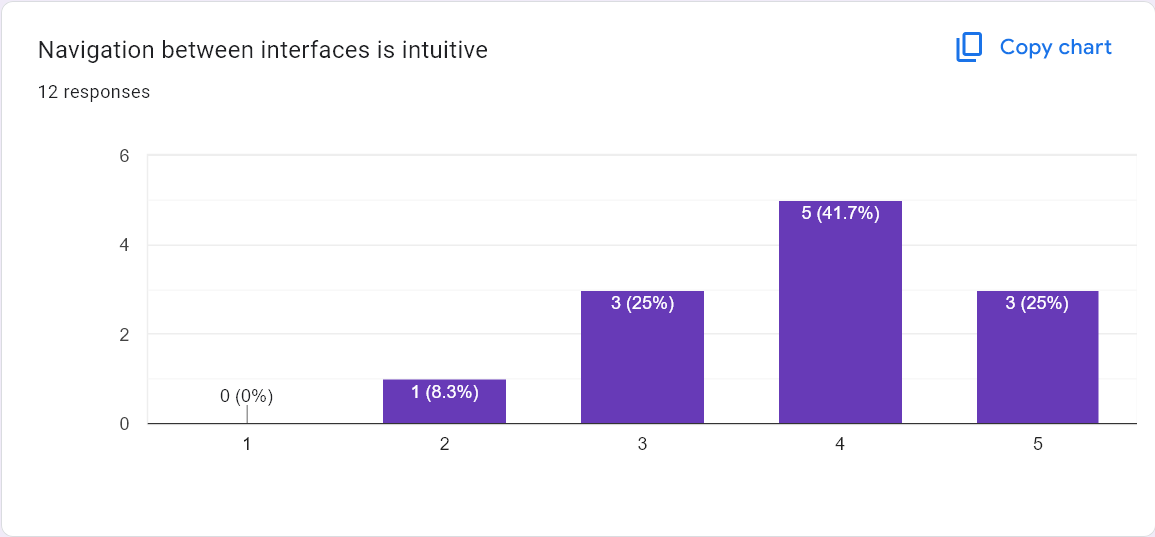
\includegraphics[scale=0.35]{./Images/Q1.png}}
  \label{fig:StraightForward}
\end{figure}

\begin{figure}[htbp]
  \caption{"Placing objects is easy" statement ratings}
  \centerline{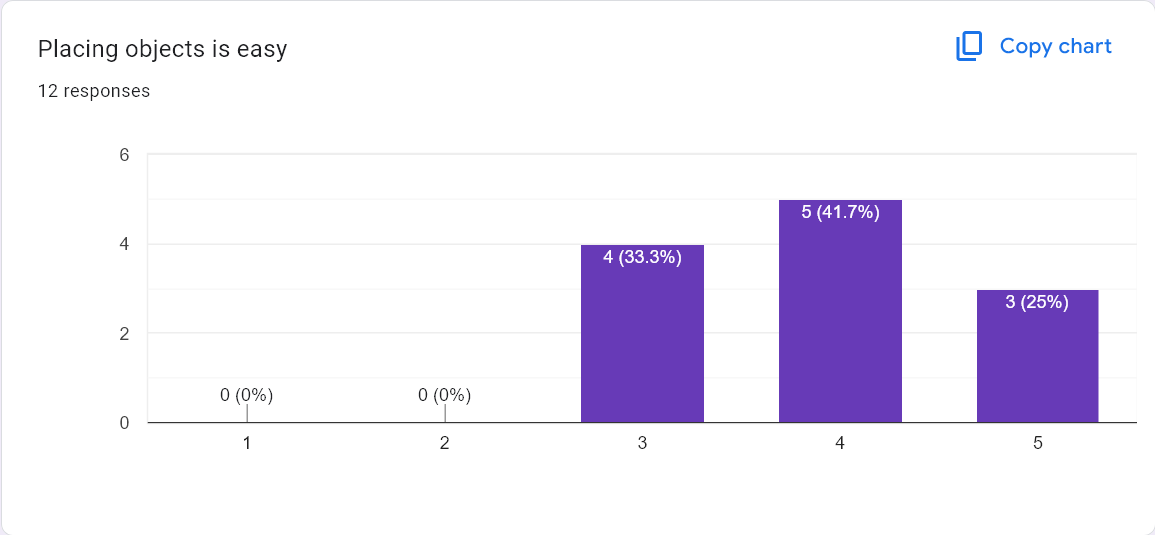
\includegraphics[scale=0.35]{./Images/Q2.png}}
  \label{fig:Navigation}
\end{figure}

\begin{figure}[htbp]
  \caption{"Generating objects is easy" statement ratings}
  \centerline{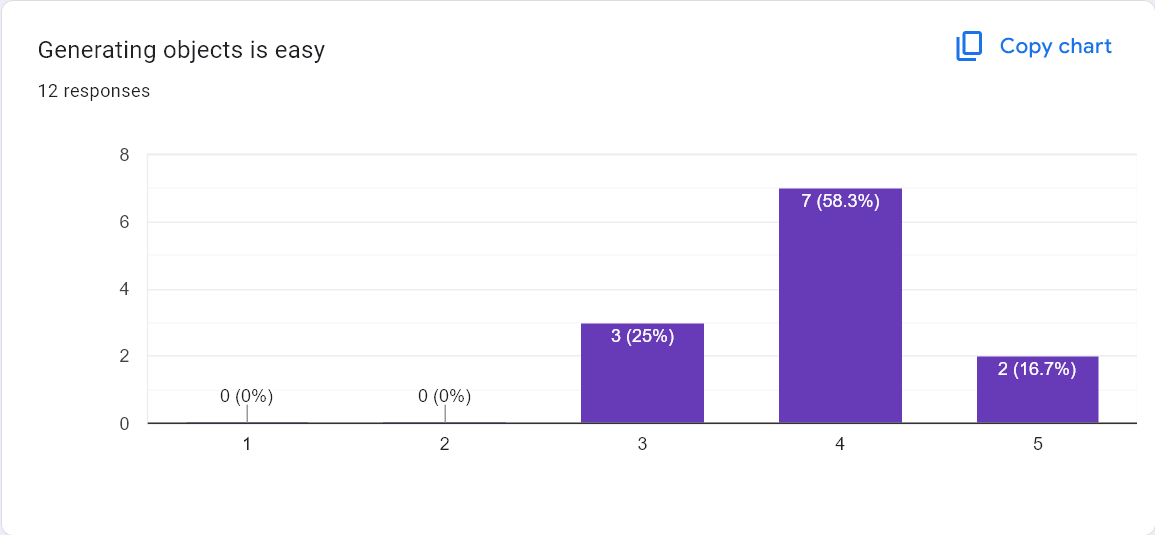
\includegraphics[scale=0.35]{./Images/Q3.png}}
  \label{fig:Detached}
\end{figure}

\begin{figure}[htbp]
  \caption{"It is easy to start a tour" statement ratings}
  \centerline{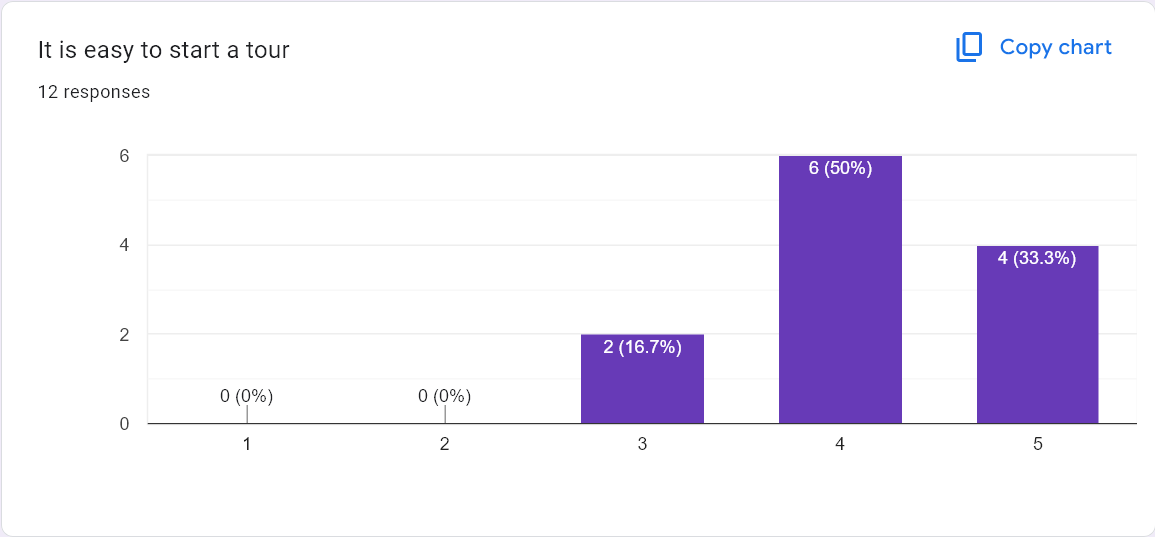
\includegraphics[scale=0.35]{./Images/Q4.png}}
  \label{fig:RealWorld}
\end{figure}

\begin{figure}[htbp]
  \caption{"Changing settings is easy" statement ratings}
  \centerline{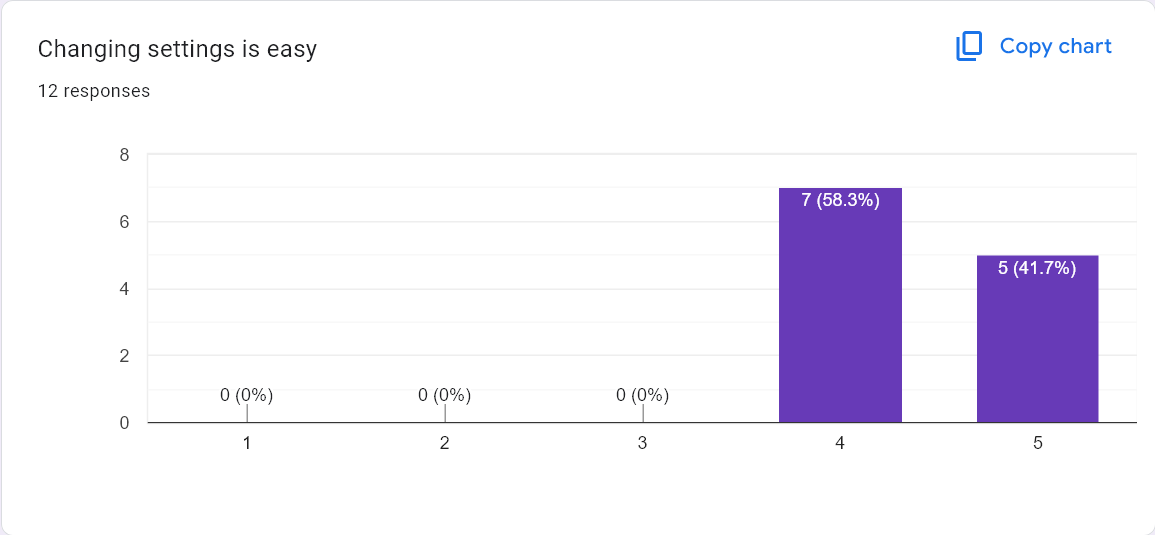
\includegraphics[scale=0.35]{./Images/Q5.png}}
  \label{fig:Fun}
\end{figure}

\begin{figure}[htbp]
  \caption{"The app is generally satisfying to use" statement ratings}
  \centerline{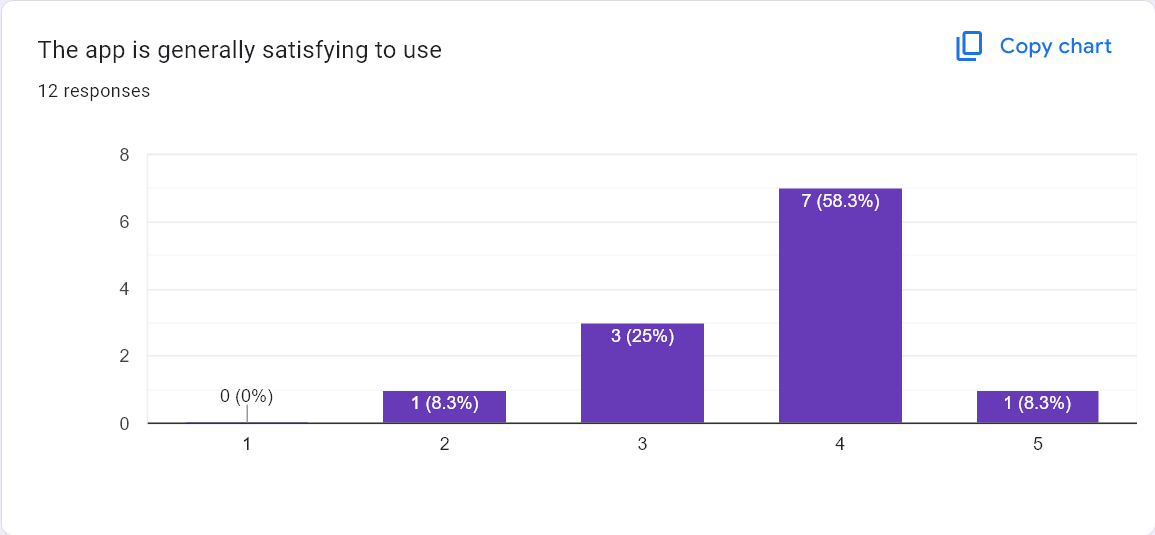
\includegraphics[scale=0.35]{./Images/Q6.png}}
  \label{fig:Social}
\end{figure}

\begin{figure}[htbp]
  \caption{"Using the app distracts from the surroundings" statement ratings}
  \centerline{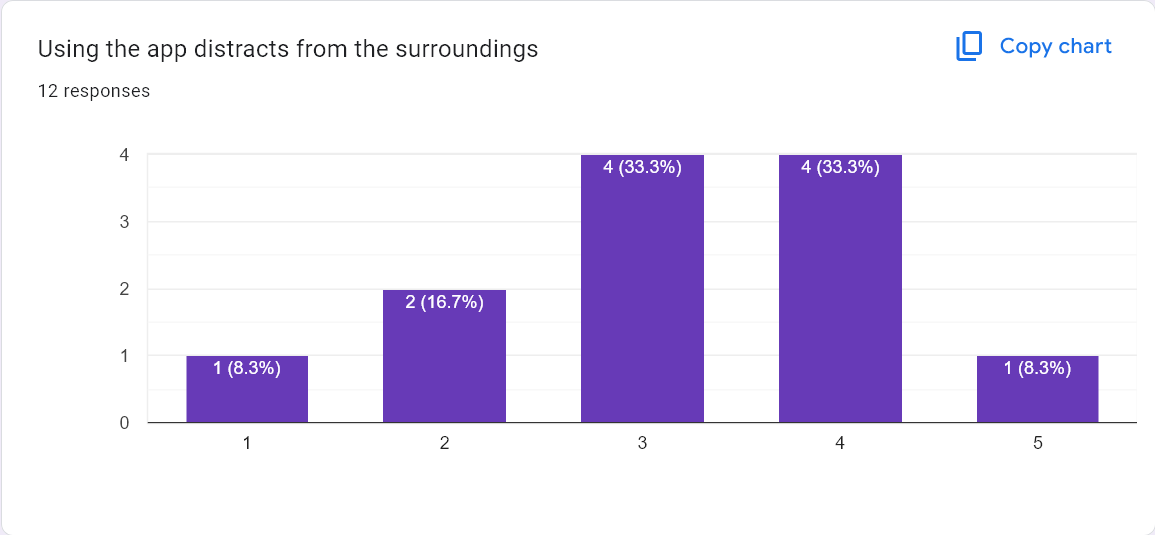
\includegraphics[scale=0.35]{./Images/Q7.png}}
  \label{fig:Enjoy}
\end{figure}

\newpage{}

\section*{Appendix --- Reflection}

The information in this section will be used to evaluate the team members on the
graduate attribute of Reflection.

The purpose of reflection questions is to give you a chance to assess your own
learning and that of your group as a whole, and to find ways to improve in the
future. Reflection is an important part of the learning process.  Reflection is
also an essential component of a successful software development process.  

Reflections are most interesting and useful when they're honest, even if the
stories they tell are imperfect. You will be marked based on your depth of
thought and analysis, and not based on the content of the reflections
themselves. Thus, for full marks we encourage you to answer openly and honestly
and to avoid simply writing ``what you think the evaluator wants to hear.''

Please answer the following questions.  Some questions can be answered on the
team level, but where appropriate, each team member should write their own
response:


\begin{enumerate}
  \item What went well while writing this deliverable?\\ \\
  The unit tests seemed fairly simple and intuitive to do and the work was split up well between the group.
  \item What pain points did you experience during this deliverable, and how
        did you resolve them?\\ \\
    Executing some of the test cases smoothly was a pain point, as well as getting them to pass, but sticking with it and sitting through them after some time, we were able to do our tests and pass them.
  \item Which parts of this document stemmed from speaking to your client(s) or
        a proxy (e.g. your peers)? Which ones were not, and why?\\ \\
        Usability survey and feedback on the app was given from peers. Since we don't have a client, a lot of our feedback was from the Professor and TA during Rev0.
  \item In what ways was the Verification and Validation (VnV) Plan different
        from the activities that were actually conducted for VnV?  If there were
        differences, what changes required the modification in the plan?  Why did
        these changes occur?  Would you be able to anticipate these changes in future
        projects?  If there weren't any differences, how was your team able to clearly
        predict a feasible amount of effort and the right tasks needed to build the
        evidence that demonstrates the required quality?  (It is expected that most
        teams will have had to deviate from their original VnV Plan.)\\ \\
        We had initially expected many of our tests to be automated, but after actually going through them, a lot of them seemed to be more manual work, such as logging in ourselves, testing out the tours, etc. We learned that many of the manual tests are moreso for the code correctness and such, and, at least for our project, the functionality had to be tested through doing.

        
\end{enumerate}

\end{document}